\documentclass[10pt,onecolumn,letterpaper]{article}

\usepackage{graphicx}
\usepackage{amsmath}
\usepackage{amssymb}
\usepackage{booktabs}
\usepackage{enumitem}
\usepackage{float}
\usepackage{fancyhdr}
\usepackage[pagebackref,breaklinks,colorlinks]{hyperref}
\usepackage{xcolor}
\usepackage{lipsum}
\usepackage{etoolbox}

% Support for easy cross-referencing
\usepackage[capitalize]{cleveref}
\crefname{section}{Sec.}{Secs.}
\Crefname{section}{Section}{Sections}
\Crefname{table}{Table}{Tables}
\crefname{table}{Tab.}{Tabs.}

\renewcommand{\footrulewidth}{0.4pt}
\renewcommand{\footrule}{\hrule width\headwidth height\footrulewidth \vskip \footruleskip}
% \definecolor{footergray}{gray}{0.5}

\makeatletter
\patchcmd{\f@nch@foot}{\rlap}{\color{gray}\rlap}{}{}
\patchcmd{\footrule}{\hrule}{\color{gray}\hrule}{}{}
\patchcmd{\@maketitle}{\raggedright}{\centering}{}{}
\patchcmd{\@maketitle}{\raggedright}{\centering}{}{}
\makeatother

%%%%%%%%% TITLE 
\title{Probabilistic Principal Component Analysis}

\begin{document}

\author{Chirag Mehta \\ \href{mailto:ai20btech11006@iith.ac.in}{ai20btech11006@iith.ac.in}}

\maketitle


%%%%%%%%% ABSTRACT
\begin{abstract}
    Principal Component Analysis (PCA) is a widely used method for analyzing and processing data, although it lacks a foundation in a probability model. In this article, we look at the utilization of maximum-likelihood estimation in a latent variable model closely linked to factor analysis to identify the principal axes of observed data vectors. We explore the characteristics of the corresponding likelihood function and highlight the benefits offered by this probabilistic approach through illustrative examples.
\end{abstract}

\thispagestyle{fancy}
\fancyfoot[C]{\small All code can be found at \href{https://github.com/cmaspi/Maths_Behind_ML/tree/main/Presentation}{\url{https://github.com/cmaspi/Maths_Behind_ML/tree/main/Presentation}}}


%%%%%%%%% BODY TEXT
\section{Introduction}

Probabilistic Principal Component Analysis (PCA) stands at the intersection of dimensionality reduction and probabilistic modeling. While traditional PCA excels at identifying key patterns in high-dimensional data, it falls short in explicitly addressing uncertainties within the observed information. In response, Probabilistic PCA introduces a probabilistic framework to the classic PCA, offering a more nuanced analysis by accounting for inherent uncertainties. This article navigates the fundamentals of Probabilistic PCA, spotlighting its capacity to model data variability in a probabilistic manner. By delving into its applications and insights, we explore how this method enhances our understanding of complex datasets and provides a robust foundation for decision-making in the face of inherent uncertainties.

\section{Mathematical Background}
\begin{itemize}
    \item Definition
    A random vector is said to be *k-variate* normally distributed if every linear combination of its k components has a univariate normal distribution.
    \item Affine Transformation
    \begin{align}
    X \sim \mathcal{N}\left(\mu, \Sigma\right)
    \end{align}
    Then
    \begin{align}
    AX+b \sim \mathcal{N}\left(A\mu+b, A\Sigma A^T\right)
    \end{align}

    \item Marginalization
    If
    \begin{align}
    X = \begin{pmatrix} X_1 \\ X_2 \end{pmatrix} \sim \mathcal{N}
    \left(
        \begin{pmatrix}\mu_1\\\mu_2\end{pmatrix},
        \begin{pmatrix}
            \Sigma_{11} & \Sigma_{12}\\
            \Sigma_{21} & \Sigma_{22}
        \end{pmatrix}
        \right)
    \end{align}
    Then
    \begin{align}
    X_1 \sim \mathcal{N}\left( \mu_1, \Sigma_{11} \right)
    \end{align}

    \item Conditioning
    If
    \begin{align}
    X = \begin{pmatrix} X_1 \\ X_2 \end{pmatrix} \sim \mathcal{N}
    \left(
        \begin{pmatrix}\mu_1\\\mu_2\end{pmatrix},
        \begin{pmatrix}
            \Sigma_{11} & \Sigma_{12}\\
            \Sigma_{21} & \Sigma_{22}
        \end{pmatrix}
        \right)
    \end{align}
    Then

    \begin{align}
        X_1 | X_2=x_2 \sim \mathcal{N}\left(\mu_1 + \Sigma_{12}\Sigma_{22}^{-1}(x_2-\mu_2),\right.
        \left.\Sigma_{11} - \Sigma_{12}\Sigma_{22}^{-1}\Sigma_{21}\right)
    \end{align}
\end{itemize}

\section{The Probability Approach}
Probabilistic PCA is defined in the following manner

\begin{align}
x &= Wz + \epsilon \\
& where \quad z \sim \mathcal{N}(0, I)\\
&\quad\quad\quad\ \ \ \epsilon \sim \mathcal{N}(0, \sigma^2 I)
\end{align}

% Notice that in this approach we use a gaussian prior over the latent variable $z$, this is because of a variety of reasons, some are listed below.
% \begin{itemize}
%     \item PPCA is a logical extension of PCA, since there are only few distributions that can be fully specified with just mean and variance.
% \end{itemize}

Probabilistic PCA can be used for majorly two tasks, that are
\begin{enumerate}
    \item $z|x$ : Dimensionality Reduction
    \item $x|z$ : Data Generation
\end{enumerate}

The next question is "how do we obtain the distributions for each of the above formulations?" The latter is straightforward to obtain.

\begin{align}
x|z \sim \mathcal{N}\left(Wz, \sigma^2 I\right)
\end{align}

Next we will find the joint distribution of $(x, z)$. We do that in the following way

\begin{align}
    p(x,z) &= p(x|z)p(z)\\
    p(x,z) & \propto \exp\left(
      \frac{-1}{2\sigma^2} \left( x-Wz\right)^T\left( x-Wz\right)
      \right) 
      \exp\left(\frac{-1}{2}z^Tz\right) \\
      & \propto \exp\left(
        \frac{-1}{2}
        \begin{bmatrix}x^T & z^T\end{bmatrix}
        \begin{bmatrix} \frac{1}{\sigma^2}I& \frac{-1}{\sigma^2}W \\
        \frac{-1}{\sigma^2}W^T & \frac{1}{\sigma^2}W^T W + I \end{bmatrix}
        \begin{bmatrix}x \\ z\end{bmatrix}
      \right)
\end{align}
Using this, we get
\begin{align}
    p(v) \propto \exp\left(\frac{-1}{2}v^T\Sigma^{-1}v\right)
\end{align}

where $v = \begin{pmatrix}x \\ z\end{pmatrix}$, $\Sigma^{-1} = \begin{bmatrix} \frac{1}{\sigma^2}I& \frac{-1}{\sigma^2}W \\
    \frac{-1}{\sigma^2}W^T & \frac{1}{\sigma^2}W^T W + I \end{bmatrix}$

The above likelihood is that of a gaussian

\begin{align}
\therefore \begin{pmatrix}x \\ z\end{pmatrix} \sim \mathcal{N}\left( 0, \Sigma \right)
\end{align}

Next, we will find the distribution for $z|x$

From Bayes Rule
\begin{align}
    p(z|x) = \frac{p(x|z)}{p(x)}p(z)
\end{align}

Using the conditioning property of gaussian distribution, we get
\begin{align}
z|x \sim \mathcal{N}\left(M^{-1}W^Tx, \sigma^2M^{-1}\right), \quad where \, M = W^TW+\sigma^2I 
\end{align}

Now that we have obtained the distributions for both $x|z$ and $z|x$, we want to obtain the matrix $W$. We form an optimization problem to achieve that. We want to maximize the likelihood of sampling the training data from the distribution of $x$. The distribution for $x$ can be obtained easily using marginalization.

\begin{align}
    x \sim \mathcal{N}\left( 0 , WW^T+\sigma^2I \right)
\end{align}

We form the optimization problem that is to maximize the log-likelihood for the training dataset.

\begin{align}
    \mathcal{L} = -\frac{N}{2}\left\{
        d\ln(2\pi)+\ln|C|+tr(C^{-1}S)
    \right\} \label{eq:L}
\end{align}
where $S = \displaystyle\frac{1}{N}\sum_{k=1}^{N}x_k x_k^T$

\begin{align}
    \frac{\partial \mathcal{L}}{\partial W} &= N\left(C^{-1}SC^{-1}W - C^{-1}W\right)\\
    &SC^{-1}W = W
\end{align}
    
Using SVD
    
\begin{align}
    SC^{-1}ULV^T = ULV^T
\end{align}

multiply by $V$ on both sides

\begin{align}
    SC^{-1}UL = UL
\end{align}

After some simplification, we obtain

\begin{align}
    SUL = U\left(L^2+\sigma^2I\right)L
\end{align}
    
For $l_j \neq 0$
\begin{align}
Su_j = \left(\sigma^2+l_j^2\right)u_j
\end{align}
Therefore, each column of $U$ must be an eigenvector of $S$, with corresponding eigenvalue $\lambda_j = \sigma^2+l_j^2$. So,

\begin{align}
l_j = (\lambda_j-\sigma^2)^{1/2} \tag{5}
\end{align}



Therefore,
\begin{align}
W = U\left(K_n-\sigma^2I\right)^{1/2}R
\end{align}

where $K_n$ is a $n\times n$ diagonal matrix

\begin{align}
k_{jj} = \begin{cases}\lambda_j & \text{eigenvalue corresponding to }u_j\\
\sigma^2 & o/w\end{cases}
\end{align}

$R$ is any rotation matrix.

\begin{align}
C &= WW^T+\sigma^2I\\
&= ULV^TVLU^T+\sigma^2I\\
&= UL^2U^T+\sigma^2I\\
|C| &= |UL^2U^T+\sigma^2I|
\end{align}

Identity: $|I+AB| = |I+BA|$
\begin{align}
    \therefore |C| = |\sigma^2I+L^2| \label{eq:det_C}
\end{align}


Using \eqref{eq:L} and \eqref{eq:det_C}

\begin{align}
    \mathcal{L} = -\frac{N}{2}\left\{d \ln(2\pi)+\frac{1}{\sigma^2}\sum_{j=1}^{q'}\ln(\lambda_j)+(d-q')ln(\sigma^2)+q' \right\}
\end{align}

Minimizing wrt $\sigma$

\begin{align}
\sigma^2=\frac{1}{d-q'}\sum_{j=q'+1}^{d}\lambda_j
\end{align}


If $\sigma^2>0$, then the $Rank(S)>n$

\begin{align}
    \mathcal{L} = -\frac{N}{2}\left\{d \ln(2\pi)+\sum_{j=1}^{q'}\ln\lambda_j+(d-q')ln\left(\frac{1}{d-q'}\sum_{j=q'+1}^{d}\lambda_j\right)+d \right\}
\end{align}


Interestingly, the minimization of $E$ only leads to the requirement of $\lambda_j$ to be adjacent in the spectrum of eigenvalues. Since the diagonal entries in $K$ have to be at least as big as $\sigma^2$, the biggest $q$ eigenvalues are considered in the $K$ matrix.

\section{Observations}

\subsection{Equivalence with PCA}
It can be seen that, when $\sigma^2 \rightarrow 0$, $M^{-1}\rightarrow(W^TW)^{-1}$.

The maximum likelihood reconstruction could be written as

\begin{align}
\tilde x &= WM^{-1}W^Tx\\
&= U\Lambda^{1/2}(\Lambda^{1/2}U^TU\Lambda^{1/2})^{-1}\Lambda^{1/2}U^Tx\\
&= UU^Tx
\end{align}

This is same as PCA (in the reconstruction sense)

\subsection{reconstruction}
When $\sigma^2 > 0$ then the latent projection becomes skewed.

$$\langle z|x \rangle = M^{-1}W^Tx$$
The above equation doesn't represent an orthogonal projection of $z$ and is therefore not optimal in squared reconstruction loss sense. However, the optimal reconstruction can still be obtained from the conditional latent mean and is given by

\begin{align}
\tilde x = W (W^TW)^{-1}M \langle z|x \rangle
\end{align}

The reconstruction obtained here would be the same as PCA. An example for this has been included in the sample notebooks.

\subsection{Data Generation}
We have already obtained distribution of $x|z$ in section 3. Using this we can generate more data. One exmaple where this would be useful is when one has limited samples of a defective class and more data is required to train a classifier, this technique could be used to generate more samples. In figure \ref{fig:data_gen}, we can see that the augmented data is similar to the actual data.

\begin{figure}
    \centering
    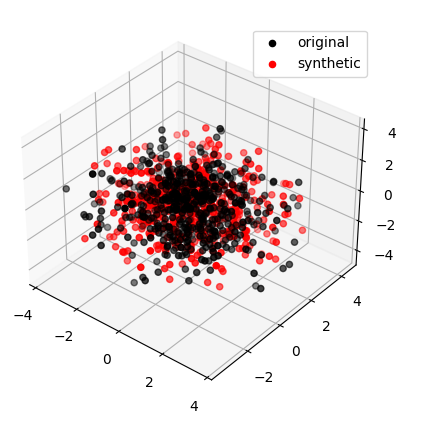
\includegraphics[width=0.5\textwidth]{./data_gen.png}
    \caption{Synthetic data generated using PPCA}
    \label{fig:data_gen}
\end{figure}

\subsection{Data Imputation}
We aren't just limited to generating entirely new data, we can also fill in the missing values for features in a given data point. This can be achieved using the conditional property of gaussians. An example for this has been included in the sample notebooks.

\section{Conclusion and Further Reading}
In this article we delved into the theory of proababilistic PCA. We saw how principal component analysis can be viewed as a maximum-likelihood procedure based on a probability density model of the observed data. We derived the closed form solution to obtain $W$. We saw that PPCA is as good as PCA in terms of reconstruction but also has the ability to generate more data and also it can be used as an imputation technique.


\subsection{Further Reading}

\begin{enumerate}
\item \href{https://www.microsoft.com/en-us/research/uploads/prod/2006/01/Bishop-Pattern-Recognition-and-Machine-Learning-2006.pdf, page: 583-586}{Heteroscedasticity: The noise doesn't follow homoscedasticity}
\item \href{https://proceedings.neurips.cc/paper_files/paper/1998/file/c88d8d0a6097754525e02c2246d8d27f-Paper.pdf}{Bayesian PCA: Find the number of components for latent space.}
\item \href{https://www.sciencedirect.com/science/article/pii/S0167947309001248}{Outlier Detection}
\end{enumerate}

% %%%%%%%%% REFERENCES
% {\small
% \bibliographystyle{ieee_fullname}
% \bibliography{egbib}
% }
\end{document}
